\hypertarget{linear-algebra-concepts}{%
\section{Linear Algebra Concepts}\label{linear-algebra-concepts}}

When we attempt to integrate multiple sensors or when we compute paths
from discrete points, the methods use the tools from linear algebra. No
attempt here is made to be complete or expository. This is intended to
review the language and concepts only. The reader who is unfamiliar with
Linear Algebra as a subject is strongly encouraged to explore
it,\footnote{Gilbert Strang - Linear Algebra, see the online text.}.
Calculus, Linear Algebra and Probability are three legs to the
mathematical stool every engineer should have.

\hypertarget{block-operations}{%
\subsection{Block operations}\label{block-operations}}

Part of the power that a course in linear systems offers is the ability
to manipulate aggregate chunks of data. We can partition the arrays into
rectangular blocks and then manipulate them in the same way as scalar
data. For example, let \(A\) be a matrix be composed of block \(B\),
vectors \(v\in{\Bbb R}^{n-1}\) and \(u\in{\Bbb R}^{m-1}\), and scalar c:

\[\begin{aligned}
A = \begin{pmatrix} B & v \\ u^T & c \end{pmatrix}
\end{aligned}\]

We can then perform blockwise matrix vector multiplication for
\(x \in {\Bbb R}^m\) with \(x = (z,t)\) and
\(z = (x_1, x_2, \dots x_{m-1})\), \(t = x_m\)

\[\begin{aligned}
Ax = \begin{pmatrix} B & v \\ u^T & c \end{pmatrix} x = \begin{pmatrix} Bz + tv \\ u^T z + ct \end{pmatrix}
\end{aligned}\]

\hypertarget{linear-systems}{%
\subsection{Linear Systems}\label{linear-systems}}

One of the most common mathematical operations is solving simultaneous
linear equations:

\[\begin{aligned}
\begin{array}{c} a_{11}x_1 + a_{12}x_2 + .... + a_{1n}x_n = b_1 \\ a_{21}x_1 + a_{22}x_2 + .... + a_{2n}x_n = b_2 \\ \vdots
\\ a_{n1}x_1 + a_{n2}x_2 + .... + a_{nn}x_n = b_n \end{array}
\end{aligned}\]

Using the matrix notation defined above we may write this in a very
compact form:

\[\Rightarrow\quad  Ax = b\]

where

\[\begin{aligned}
A = \left( \begin{array}{ccc}a_{11}&\dots&a_{1n}\\ \dots & \dots & \dots
\\ a_{n1} & \dots & a_{nn}\end{array}\right), \quad x = \left(\begin{array}{c} x_1 \\ x_2 \\ \vdots
\\ x_n \end{array}\right) , \quad
b =  \left(\begin{array}{c} b_1 \\ b_2 \\ \vdots
\\ b_n \end{array}\right) .
\end{aligned}\]

One approach to solve the equations is \texttt{Gaussian\ Elimination}.
The industry version of Gaussian Elimination is the
\texttt{LU\ factorization}. An LU factorization decomposes the matrix
\(A\) into the product of a lower triangular matrix, \(L\), and an upper
triangular matrix, \(U\). The strength of this approach is that the LU
factorization is done for \(A\) once. Once done, solving \(Ax = b\) for
different \(b\)'s can be done relatively easily. You don't actually have
to know how to do this, only how to call the system solvers.

\hypertarget{inverses}{%
\subsubsection{Inverses}\label{inverses}}

The inverse of \(A\) is notated \(A^{-1}\):

\[A(A^{-1}) = I =
(A^{-1})A\]

Given the inverse:

\[Ax=b \to x = A^{-1}b\]

Is this a good approach to solving \(Ax=b\)?

No. The fast multiplication algorithms are not numerically stable. Best
to use a Gauss-Jordan based approach like the LU factorization. LU can
also make good use of matrix structure. Possible that an algorithm may
list an inverse, but this can often be converted to a linear solve. For
example if the formula lists \(y^* = y + BC^{-1}x\), then solve
\(Cz = x\) first and then find \(y^*=y+Bz\).

If \(x, y\in {\mathbb R}^n\) are vectors, and \(a, b\in {\mathbb R}\)
are real numbers, we say that \(ax+by\) is a \emph{linear combination}
of \(x\) and \(y\). Over all possible values for \(a\) and \(b\), we say
\(ax+by\) is a span of \(x\) and \(y\). Spanning sets arise in all sort
of applications. It is a way to decompose sets into basic components.
For example, the span of \(x = \left< 1, 0 \right>\) and
\(y = \left< 0, 1 \right>\) is the plane and the vectors \(x\) and \(y\)
are a known as a \texttt{basis}. The term basis is a minimal spanning
set and the number of linear independent basis elements is the
dimension. More information on these ideas can be found in most linear
algebra textbooks.

We can represent a line through the origin by
\(t \left< a  , b \right>\)

where \(t\in {\mathbb R}\) (\(t\) is the scale factor). Geometrically we
are scaling the vector into spanning a line. The vector we are using is
\(\left< a  , b \right>\). Another example is the collection of all
\(2\times 2\) matrices:

\[\begin{aligned}
\begin{pmatrix} a & b \\ c & d\end{pmatrix}
\end{aligned}\]

which is the linear combination of

\[\begin{aligned}
\begin{pmatrix} 1 & 0 \\ 0 & 0\end{pmatrix},
\begin{pmatrix} 0 & 1 \\ 0 & 0\end{pmatrix},
\begin{pmatrix} 0 & 0 \\ 1 & 0\end{pmatrix},
\begin{pmatrix} 0 & 0 \\ 0 & 1\end{pmatrix}.
\end{aligned}\]

One consequence of these ideas is that of a \texttt{vector\ space}. It
is the span of a collection of vectors (or all linear combinations of
the vectors). More formally, \(V\) is a vector space if \(x, y\in V\)
are vectors, and \(a, b\in {\mathbb R}\), then \(ax+by \in V\).

The two examples above are vector spaces: the line through the origin
and the collection of \(2\times 2\) matrices. Note that in the figure
below, the solid line is a vector space is, and the dotted is not. A
vector space must include the zero element and the dotted line does not.

\leavevmode\hypertarget{fig:lineisnotalwaysvectorspace}{}%
\begin{figure}
\centering
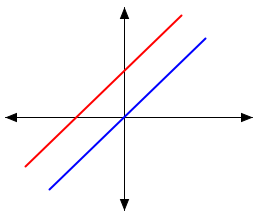
\includegraphics[width=0.4\textwidth,height=\textheight]{MathFigures/lines.*}
\caption{}
\end{figure}

A \texttt{subspace} is a subset of a vector space \(V\) that is also a
vector space. For example, a line through the origin is a subspace of
the plane. Also, a plane through the origin is a subspace of three
space, such as the span of

\[\begin{aligned}
\left\{\begin{pmatrix} 1 \\ 0 \\ 0\end{pmatrix},
\begin{pmatrix} 0 \\ 1 \\ 0\end{pmatrix}\right\}.
\end{aligned}\]

The reason these concepts are discussed is that when solving linear
systems or doing least squares (optimization), you are often working
with vector spaces and subspaces. The literature uses this terminology
and the concepts have a very rich geometric structure which can be
helpful in understanding the problems.

A very well studied subspace is the \emph{Nullspace} of a matrix, \(N\).
It is defined as all \(w\) such that \(Aw=0\). Note that if \(Au=0\) and
\(Av=0\) then

\[A(cu+dv) = cAu + dAv = c(0) + d(0) = 0\]

thus it is correctly called a subspace. Also, \(u=0\) is trivially in
the nullspace. If a matrix has a nullspace, then the associated linear
systems problem \(Ax = b\) will not have a unique solution which is
important to know if you need a solution to your problem.

An example of this issue is if you wanted to solve \(Ax = b\) where

\[\begin{aligned}
A = \begin{pmatrix} 1 & 0 & -1\\ 0 & 0 & 0 \\ 0 & 0 & 0\end{pmatrix},
\quad b = \begin{pmatrix} 1  \\ 0 \\ 0\end{pmatrix} .
\end{aligned}\]

Can this be solved for \(x\)? In this trivial example you can see that
it can be and \(x = \left< 1, 0 , 0\right>\) works. However the solution
is not unique. Without going into the details, we see that there are two
vectors which span the Nullspace:

\[\begin{aligned}
v_1 = \begin{pmatrix} 1  \\ 0 \\ 1\end{pmatrix},
\quad v_2 = \begin{pmatrix} 0  \\ 1 \\ 0\end{pmatrix}
\end{aligned}\]

i.e. \(Av_1 = 0\) and \(Av_2 = 0\). So we actually gain a two
dimensional family of solutions (meaning a plane)

\[\begin{aligned}
x = \begin{pmatrix} 1  \\ 0 \\ 0\end{pmatrix} + c_1\begin{pmatrix} 1  \\ 0 \\ 1\end{pmatrix}  +  c_2\begin{pmatrix} 0  \\ 1 \\ 0\end{pmatrix}
\end{aligned}\]

Another popular subspace is known as the \emph{Column Space}. It is the
span of the columns (treated as vectors) of \(A\). This tells you the
range space of the matrix. Using the last \(A\) as the working example:

\[\begin{aligned}
A = \begin{pmatrix} 1 & 0 & -1\\ 0 & 0 & 0 \\ 0 & 0 & 0\end{pmatrix}
\end{aligned}\]

the range is given by the span of the columns. So we have

\[\begin{aligned}
\left\{\begin{pmatrix} 1 \\ 0\\ 0\end{pmatrix}\right\}
\end{aligned}\]

Note that a similar notion is the span of the rows, called the \emph{Row
Space}.

\hypertarget{eigenvalues-and-eigenvectors}{%
\subsection{Eigenvalues and
Eigenvectors}\label{eigenvalues-and-eigenvectors}}

Let \(x\) solve \(Ax=\lambda x\) (the invariant directions problem).

\[Ax-\lambda x=0 \quad\Rightarrow\quad (A-\lambda I)x=0\quad \Rightarrow \quad x\in {\cal N}(A-\lambda I)\]

The latter saying that \(x\) must be in the Nullspace of
\(A-\lambda I\). This implies the following polynomial equation which is
solved for roots \(\lambda\).

\[\det (A-\lambda I)=0 \quad \Rightarrow \quad \lambda\]

We can numerically solve for \((\lambda , x)\) and these are known as an
eigenvalue, eigenvector pair. An example of the SciPy eigenvalue solver
is given below.

\hypertarget{eigenvalues-for-symmetric-matrices}{%
\subsubsection{Eigenvalues for Symmetric
Matrices}\label{eigenvalues-for-symmetric-matrices}}

Assume that \(A\) is a real symmetric matrix and that \((\lambda, v)\)
is an eigenvalue, eigenvector pair. If \(v\) is complex valued then
\(\| v \|^2 = v \cdot \bar{v}\) where \(\bar{v}\) is the complex
conjugate of \(v\). Then we have

\[\lambda \| v \|^2 =  \lambda v \cdot \bar{v} = Av  \cdot \bar{v} = v \cdot A \bar{v} =  v \cdot  \overline{Av} =  v \cdot  \overline{\lambda v}  = \bar{\lambda} v \cdot \bar{v} = \bar{\lambda} \| v \|^2\]

So this implies that \(\lambda = \bar{\lambda}\) or that \(\lambda\) is
real valued.

\hypertarget{orthogonal}{%
\subsection{Orthogonal}\label{orthogonal}}

The last concept we will review is orthogonality. The basic term means
perpendicular. Two vectors, \(x\) and \(y\) are said to be orthogonal if
their dot product is zero:

\[x\cdot y =0.\]

A matrix, \(Q\), is said to be orthogonal if its columns treated as
vectors are mutually orthogonal and of unit length. This turns out to be
mathematically equivalent to a matrix satisfying

\[QQ^T = I\]

where \(I\) is the identity matrix. We will see orthogonal matrices
later when we compute rotations in space. These matrices will be the
foundations of the coordinate transformations used in robotic arms.

\hypertarget{the-pseudo-inverse}{%
\subsection{The Pseudo-Inverse}\label{the-pseudo-inverse}}

We will at several occasions run into the problem of solving what is
known as the \emph{overdetermined} problem. This is the linear systems
problem for which there are more equations than there are unknowns
(variables).

The problem is then

\[\begin{aligned}
\begin{array}{c} a_{11}x_1 + a_{12}x_2 + .... + a_{1n}x_n = b_1 \\ a_{21}x_1 + a_{22}x_2 + .... + a_{2n}x_n = b_2 \\ \vdots
  \\ a_{m1}x_1 + a_{m2}x_2 + .... + a_{mn}x_n = b_m \end{array}, m > n
\end{aligned}\]

Just as before we can use the matrix notation to write this in a very
compact form:

\[\Rightarrow\quad  Ax = b\]

where

\[\begin{aligned}
A = \left( \begin{array}{ccc}a_{11}&\dots&a_{1n}\\ \dots & \dots & \dots
  \\ a_{m1} & \dots & a_{mn}\end{array}\right), \quad x = \left(\begin{array}{c} x_1 \\ x_2 \\ \vdots
  \\ x_n \end{array}\right) , \quad
  b =  \left(\begin{array}{c} b_1 \\ b_2 \\ \vdots
  \\ b_m \end{array}\right) .
\end{aligned}\]\[Overdetermined System of Equations\]

This leads to a non-square matrix which is not invertible. There is no
exact solution: \(Ax \neq b\) for all possible \(x\) in this case. So
instead of trying to solve the problem exactly, we ask about getting as
close as possible. In other words, this problem is not solvable by
regular methods such as the LU factorization or Gauss-Jordan
elimination, but can be addressed by minimizing the error using the
method of least squares.

The columns must be linearly independent for this method to succeed so
we assume that for now. With the columns linearly independent, the core
issue geometrically is that the vector \(b\) is not in the span of the
columns of \(A\). The best we can ask is to get as close as possible.
Thus we optimize:

\[\min \| Ax - b\|\]

where we will call the minimizer \(\hat{x}\). To minimize we express the
norm as a matrix multiply:

\[\| Ax - b\|^2 =  (Ax - b)^T(Ax - b) =  (Ax)^T(Ax) - b^T(Ax) -  (Ax)^Tb +  b^Tb .\]

Note that \(b^TAx  =  (Ax)^Tb\), and \((Ax)^T = x^TA^T\), so we have

\[\| Ax - b\|^2 = x^TA^T Ax -2x^TA^Tb  +   b^Tb.\]

Next we form the gradient of the norm with respect to \(x\). We leave to
a homework to show \(\nabla [x^TA^T Ax] = 2 A^TAx\) and
\(\nabla [x^TA^Tb] = A^T b\). Then we have

\[\nabla \| Ax - b\|^2 = 2 A^TAx  - 2A^T b  .\]

To find the minimizer, set \(\nabla \| Ax - b\|^2 = 0\) so we obtain

\[A^TA\hat{x}  = A^T b .\]

These are known as the \emph{Normal Equations}.

The matrix \(A^T A\) is symmetric and if the columns of \(A\) are
linearly independent, then \(A^T A\) is invertible. This yields the
solution

\[\hat{x} = \left( A^T A\right)^{-1} A^T b .\]

This formula is known by several names. It is called the
\texttt{Pseudo-Inverse} or \texttt{Moore-Penrose} Pseudo-Inverse. It is
also called the left-sided pseudo-inverse (because it acts on the left
side).

\textbf{Example} Find the least squares solution to

\[\begin{aligned}
\begin{pmatrix} 1 & 0 \\ 1 & 1 \\ 0 & 2 \end{pmatrix}\begin{pmatrix} x_1 \\ x_2 \end{pmatrix} = \begin{pmatrix} 1 \\ 2 \\ 1 \end{pmatrix}
\end{aligned}\]

Forming the normal equations

\[\begin{aligned}
\begin{pmatrix} 1 & 1 & 0 \\ 0 & 1 & 2 \end{pmatrix}
 \begin{pmatrix} 1 & 0 \\ 1 & 1 \\ 0 & 2 \end{pmatrix}\begin{pmatrix} x_1 \\ x_2 \end{pmatrix} = \begin{pmatrix} 1 & 1 & 0 \\ 0 & 1 & 2 \end{pmatrix}
 \begin{pmatrix} 1 \\ 2 \\ 1 \end{pmatrix}
\end{aligned}\]

and multiplying out

\[\begin{aligned}
\begin{pmatrix} 2 & 1 \\ 1 & 5 \end{pmatrix}\begin{pmatrix} x_1 \\ x_2 \end{pmatrix} = \begin{pmatrix} 3 \\ 4 \end{pmatrix} .
\end{aligned}\]

Solving the two by two system, we obtain

\[\begin{aligned}
\begin{pmatrix} x_1 \\ x_2 \end{pmatrix} = \begin{pmatrix} \frac{11}{9} \\[1mm] \frac{5}{9} \end{pmatrix} .
\end{aligned}\]

Does this actually solve the problem?

\[\begin{aligned}
\begin{pmatrix} 1 & 0 \\ 1 & 1 \\ 0 & 2 \end{pmatrix}\begin{pmatrix} \frac{11}{9} \\[1mm] \frac{5}{9} \end{pmatrix} = \begin{pmatrix}  \frac{11}{9} \\[1mm] \frac{16}{9}\\[1mm]  \frac{10}{9} \end{pmatrix} \neq  \begin{pmatrix} 1 \\ 2 \\ 1 \end{pmatrix}
\end{aligned}\]

It does not solve the problem. What about residual (error)?

\[\begin{aligned}
\| \begin{pmatrix}  \frac{11}{9} \\[1mm] \frac{16}{9}\\[1mm]  \frac{10}{9} \end{pmatrix} -  \begin{pmatrix} 1 \\ 2 \\ 1 \end{pmatrix} \| = \sqrt{(2/9)^2 + (2/9)^2 + (1/9)^2} = 1/9
\end{aligned}\]

Can we do any better? For any value \(x = \left< x_1, x_2\right>\), is
it possible for

\[\begin{aligned}
\|  \begin{pmatrix} 1 & 0 \\ 1 & 1 \\ 0 & 2 \end{pmatrix}u -  \begin{pmatrix} 1 \\ 2 \\ 1 \end{pmatrix} \| < 1/9?
\end{aligned}\]

We will minimize the square of the norm to avoid issues with the square
root. The first derivatives must be zero and we apply the second
derivative test if the error is a minimum.

\[f(x_1,x_2) = (x_1 - 1)^2 + (x_1+x_2 - 2)^2 + (2x_2-1)^2\]

\[f_{x_1} = 2(x_1-1)  + 2(x_1+x_2-2), \quad f_{x_2} =  2(x_1+x_2-2) + 4(2x_2-1)\]

We see that

\[f_{x_1}(11/9, 5/9) = 0, \quad  f_{x_2} (11/9, 5/9) = 0\]

and

\[f_{x_1x_1} = 4, \quad f_{x_2x_2} =  10, \quad f_{x_1x_2} =2\]

The second derivative test gives \(D = 40- 4=36\) which means our
surface is curved up at the critical point and thus \((11/9, 5/9)\) is a
local min. The function \(f\) is a parabolic surface and so
\((11/9, 5/9)\) is the global min. Meaning it is the best that we can
do.

The other variation of the non-square linear system is the
\emph{underdetermined} problem. In this case we have more columns than
rows and so has the structure shown in Figure~
\texttt{Fig:underdetermined}

\begin{quote}
An underdetermined system
\end{quote}

The columns cannot be linearly independent and so \(A^TA\) is not
invertible which means the left sided pseudo-inverse
\(\left(A^TA\right)^{-1}\) does not exist. So, we need to go another
route.

This time instead of assuming the columns are linearly independent we
will assume the rows are linearly independent. So although \(A^T A\) is
not invertible, we have that \(\left(A A^T\right)\) is of full rank, or
invertible. Using \(\left(A A^T\right)\) on the right side gives us the
result. Admittedly this version is less intuitive.

\[Ax = b \quad\Rightarrow\quad   Ax = I b\]

\[A x = \left(A A^T\right) \left(A A^T\right)^{-1} b\]

\[Ax = AA^T \left(A A^T\right)^{-1} b\]

\[\hat{x} = A^T \left(A A^T\right)^{-1} b\]

Note: the assumption that the rows are linearly independent is critical.
If they are not, then you will find that \(A A^T\) is still not
invertable. In practice, you need to row reduce the system until what
you have is a set of linearly independent rows. Example:

\[\begin{aligned}
\begin{pmatrix} 1 & 2 \\ 2 & 4 \end{pmatrix}
\end{aligned}\]

should be row reduced to

\[\begin{pmatrix} 1 & 2  \end{pmatrix}\]

\hypertarget{pseudo-inverse-formulas}{%
\subsubsection{Pseudo-Inverse Formulas}\label{pseudo-inverse-formulas}}

\begin{enumerate}
\item
  Left Moore-Penrose Pseudo-Inverse (\(A\) has linearly independent
  columns): \(A^+ = \left(A^TA\right)^{-1} A^T :\) \(A^+ A =I\)

  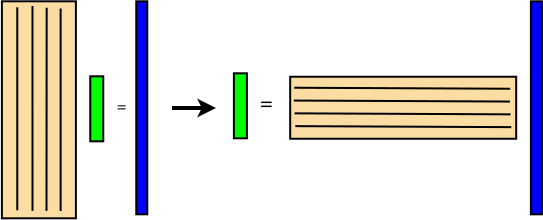
\includegraphics[width=0.75\textwidth,height=\textheight]{MathFigures/vrectsoln.*}
\item
  Right Moore-Penrose Pseudo-Inverse (\(A\) has linearly independent
  rows): \(A^+ = A^T \left(AA^T\right)^{-1}:\) \(A A^+ =I\)

  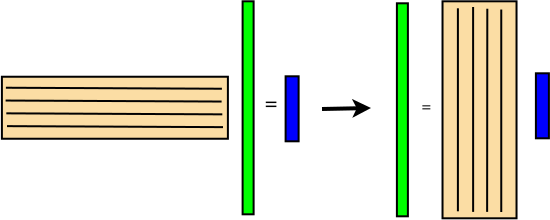
\includegraphics[width=0.75\textwidth,height=\textheight]{MathFigures/hrectsoln.*}
\end{enumerate}

\hypertarget{singular-value-decomposition}{%
\subsection{Singular Value
Decomposition}\label{singular-value-decomposition}}

For the normal equations to be invertible the columns of the matrix
\(A\) must be linearly independent, meaning as vectors they point in
different directions. This is fine in the theoretical context, but in
practice a data set can produce columns which point in similar
directions. This can cause problems with the accuracy of the solution to
the normal equations. In addition, the product of \(A\) times the
transpose of \(A\) can increase the ill-conditioning of the matrix.

The standard method to address numerical problems such as this is to
compute the pseudo-inverse through the
\texttt{Singular\ Value\ Decomposition} (SVD). We will present the SVD
first and then show how it applies to the pseudo-inverse.

(details needed here) The SVD of \(A = U \Sigma V^T\). \(U,V\) are
orthogonal. \(\Sigma\) is diagonal. Since \(U\) and \(V\) are
orthogonal, the inverse is given by the transpose \(U^{-1} = U^T\). The
matrix \(\Sigma\) is diagonal, but not square and can have zero elements
on the diagonal. We can define a pseudo-inverse by inverting the
non-zero digonal elements (leaving the zero elements).

\[\begin{aligned}
\Sigma^+ = \begin{pmatrix} 1/\sigma_1 & 0 & \dots & 0 \\
           0 & 1/\sigma_2 & \dots & 0 \\
           \vdots & \vdots & \ddots & \vdots \\
           0 & \dots & 0 & 0 
           \end{pmatrix}
\end{aligned}\]

The pseudo-inverse of \(A\) is \(A^+ = V \Sigma^+ U^T\).

Note that the SVD pseudo-inverse has one formulation which makes it a
nice for applications which may be deficient in both row and column
rank. For bth underdetermined and overdetermined problems

\[Ax = b \quad \Rightarrow \quad x = A^+ b = V \Sigma^+ U^T b\]

\hypertarget{weighted-least-squares}{%
\subsection{Weighted Least Squares}\label{weighted-least-squares}}

Traditional least squares is formulated by minimizing using the normal
\texttt{inner\ product}:

\[x^Ty = \sum_i x_iy_i.\]

Let \(x, y\in R^n\). No weights are referred to as uniform weighting.
Non-uniform weights are just termed as weights. If the inner product is
weighted:

\[\left< x, y \right> = \sum_{i=1}^n x_i y_i q_i = x^T Q y\]

where \(Q\) is a \(n \times n\) square matrix then what is

least squares solution to \(A x = b\)? One simple modification to the
previous least squares process is required. We multiply both sides by
the weight matrix \(Q\):

\[QAx= Qb\]

then follow the earlier derivation:

\[A^T QAx = A^T Qb .\]

Assuming that \(A^T Q A\) is full rank,

\[x = \left(A^T Q A\right)^{-1} A^TQb .\]

The matrix \(Q\) is any matrix for which the inner product above is a
valid. However, we will often select \(Q\) as a diagonal matrix
containing the reciprocals of the variances (the reason shown below in
the covariance computation):

\[\begin{aligned}
Q =
\begin{pmatrix} q_1 & 0 & \dots & 0 & 0   \\
0 & q_2 & \dots & 0 & 0   \\
&& \ddots  &&\\
0 & 0 & 0 & q_{n-1} & 0   \\
0 & 0 & 0 & 0 & q_n
\end{pmatrix}
=
\begin{pmatrix} 1/\sigma_1^2 & 0 & \dots & 0 & 0   \\
0 & 1/\sigma_2^2 & \dots & 0 & 0   \\
&& \ddots  &&\\
0 & 0 & 0 & 1/\sigma_{n-1}^2 & 0   \\
0 & 0 & 0 & 0 & 1/\sigma_n^2
\end{pmatrix} .
\end{aligned}\]

Assume that you have an \(x\)-\(y\) data set,
Figure~\texttt{Fig:weightedLSdata}. Using the process above we compute
the uniformly weighted least squares fit to a line, shown in blue, and
the weighted least squares fit to a line, shown in green,
Figure~\texttt{Fig:weightedLSplot}. The weight function weights more
heavily towards the origin (using \(w_i = 1.0/i^3\)). In this example,
the weights are scaled so the sum of the weights is one.

\textbf{Footnotes}
